\fancyhead[RO,LE]{\textit{Burial of the Dead}}
\fancyhead[RE,LO]{\textit{}}
%This rite is revised, in accordance with the Observations, in light of A Manual for Priests.
\section{The Order for the Burial of the Dead}

\subsection{Reception of the Body}
%Clearer rubric from 1928 English BCP:
\begin{secrubric}
    The Priest, meeting the Body at the entrance of the church yard, and prior to going before it either into the church or towards the grave, shall say or sing,\par
    \textsc{Note,} The Priest should be vested in surplice and black stole, and also, on more solemn occasions, in black cope.
\end{secrubric}
\lett{I}{am} the resurrection and the life, saith the Lord: he that believeth in me, though he were dead, yet shall he live: and whosoever liveth and believeth in me, shall never die.\par
    \secondline{I know that my redeemer liveth, and that he shall stand at the latter day upon the earth: and though this body be destroyed, yet shall I see God: whom I shall see for myself, and mine eyes shall behold, and not as a stranger.}
    \thirdline{We brought nothing into this world, and it is certain we can carry nothing out. The \divineName{Lord} gave, and the \divineName{Lord} hath taken away; blessed be the name of the \divineName{Lord}.}

\subsection{Procession}
\begin{rubric}
	A Clerk carrying the Cross goes before (and, on more solemn occasions, with two acolytes with candles), accompanied by another bearing Holy Water. As the Ministers and Clerks proceed into the Church, the following Responsory is begun.
\end{rubric}

\subsubsection{Subvenite}
\lett{C}{ome} to \textit{his} aid, ye Saints of God, come to meet \textit{him}, ye Angels of the Lord. Receiving \textit{his} soul, offering it in the sight of the Most High.\par
\secondline{℣. May Christ receive thee, who hath called thee: and may the Angels lead thee unto Abraham's bosom.}
\thirdline{℟. Receiving \textit{his} soul, offering it in the sight of the Most High.}
℣. Rest eternal grant unto \textit{him}, O Lord: and let light perpetual shine upon \textit{him}.\par
℟. Offering it in the sight of the Most High.

\begin{rubric}
	The Coffin is set down in the midst of the Church, so that the feet of the departed, unless he be a Priest, are toward the High Altar; but if he be a Priest, his head is toward the Altar. Then Candles should be lighted about the Body.
\end{rubric}

\subsection{Service in the Church}
\begin{rubric}
%Addition of prayers for the dead and traditional replacement of the Gloria Patri in Requiem contexts.
    After they are come into the Church, and the Responsory hath been said, then shall be said one or more or the following Selections, taken from the Psalms. Instead of the \blackrubric{Gloria Patri} shall be said the following at the end of each Psalm.
\end{rubric}
℣. Rest eternal * grant unto them, O Lord.\par
℟. And let light perpetual * shine upon them.\par\noindent

\subsubsection{Psalm 39. \textit{Dixi, Custodiam}}
\lett{L}{ord,} let me know mine end, and the number of my days : that I may be certified how long I have to live.\par
\secondline{\psanum{6}Behold, thou hast made my days as it were a span long : and mine age is even as nothing in respect of thee; and verily every man living is altogether vanity.}
\thirdline{\psanum{7}For man walketh in a vain shadow, and disquieteth himself in vain : he heapeth up riches, and cannot tell who shall gather them.}
\psanum{8}And now, Lord, what is my hope : truly my hope is even in thee.\par
\psanum{9}Deliver me from all mine offences : and make me not a rebuke unto the foolish.\par
\psanum{10}I became dumb, and opened not my mouth : for it was thy doing.\par
\psanum{11}Take thy plague away from me : I am even consumed by the means of thy heavy hand.\par
\psanum{12}When thou with rebukes dost chasten man for sin, thou makest his beauty to consume away, like as it were a moth fretting a garment : every man therefore is but vanity.\par
\psanum{13}Hear my prayer, O Lord, and with thine ears consider my calling : hold not thy peace at my tears.\par
\psanum{14}For I am a stranger with thee : and a sojourner, as all my fathers were.\par
\psanum{15}O spare me a little, that I may recover my strength : before I go hence, and be no more seen.\par

\subsubsection{Psalm 90. \textit{Domine, refugium}}
\lett{L}{ord,} thou hast been our refuge : from one generation to another.\par
%Third line too long:
\secondline{\psanum{2}Before the mountains were brought forth, or ever the earth and the world were made : thou art God from everlasting, and world without}
\noindent
end.\par
\psanum{3}Thou turnest man to destruction : again thou sayest, Come again, ye children of men.\par
\psanum{4}For a thousand years in thy sight are but as yesterday : seeing that is past as a watch in the night.\par
\psanum{5}As soon as thou scatterest them they are even as a sleep : and fade away suddenly like the grass.\par
\psanum{6}In the morning it is green, and groweth up : but in the evening it is cut down, dried up, and withered.\par
\psanum{7}For we consume away in thy displeasure : and are afraid at thy wrathful indignation.\par
\psanum{8}Thou hast set our misdeeds before thee : and our secret sins in the light of thy countenance.\par
\psanum{9}For when thou art angry all our days are gone : we bring our years to an end, as it were a tale that is told.\par
\psanum{10}The days of our age are threescore years and ten; and though men be so strong that they come to fourscore years : yet is their strength then but labour and sorrow; so soon passeth it away, and we are gone.\par
\psanum{11}But who regardeth the power of thy wrath : for even thereafter as a man feareth, so is thy displeasure.\par
\psanum{12}So teach us to number our days : that we may apply our hearts unto wisdom.\par

\subsubsection{Psalm 27. \textit{Dominus illuminatio}}
\lett{T}{he} Lord is my light and my salvation ; whom then shall I fear : the Lord is the strength of my life; of whom then shall I be afraid?\par
\secondline{\psanum{2}When the wicked, even mine enemies and my foes, came upon me to eat up my flesh : they stumbled and fell.}
\thirdline{\psanum{3}Though an host of men were laid against me, yet shall not my heart be afraid : and though there rose up war against me, yet will I put my trust in him.}
\psanum{4}One thing have I desired of the Lord, which I will require : even that I may dwell in the house of the Lord all the days of my life, to behold the fair beauty of the Lord, and to visit his temple.\par
\psanum{5}For in the time of trouble he shall hide me in his tabernacle : yea, in the secret place of his dwelling shall he hide me, and set me up upon a rock of stone.\par
\psanum{6}And now shall he lift up mine head : above mine enemies round about me.\par
\psanum{7}Therefore will I offer in his dwelling an oblation with great gladness : I will sing, and speak praises unto the Lord.\par
\psanum{8}Hearken unto my voice, O Lord, when I cry unto thee : have mercy upon me, and hear me.\par
\psanum{9}My heart hath talked of thee, Seek ye my face : Thy face, Lord, will I seek.\par
\psanum{10}O hide not thou thy face from me : nor cast thy servant away in displeasure.\par
\psanum{11}Thou hast been my succour : leave me not, neither forsake me, O God of my salvation.\par
\psanum{12}When my father and my mother forsake me : the Lord taketh me up.\par
\psanum{13}Teach me thy way, O Lord : and lead me in the right way, because of mine enemies.\par
\psanum{14}Deliver me not over into the will of mine adversaries : for there are false witnesses risen up against me, and such as speak wrong.\par
\psanum{15}I should utterly have fainted : but that I believe verily to see the goodness of the Lord in the land of the living.\par
\psanum{16}O tarry thou the Lord's leisure : be strong, and he shall comfort thine heart; and put thou thy trust in the Lord.\par

\subsubsection{Psalm 46. \textit{Deus noster refugium}}
\lett{G}{od} is our hope and strength : a very present help in trouble.\par
\secondline{\psanum{2}Therefore will we not fear, though the earth be moved : and though the hills be carried into the midst of the sea;}
\thirdline{\psanum{3}Though the waters thereof rage and swell : and though the mountains shake at the tempest of the same.}
\psanum{4}The rivers of the flood thereof shall make glad the city of God : the holy place of the tabernacle of the most Highest.\par
\psanum{5}God is in the midst of her, therefore shall she not be removed : God shall help her, and that right early.\par
\psanum{6}The heathen make much ado, and the kingdoms are moved : but God hath shewed his voice, and the earth shall melt away.\par
\psanum{7}The Lord of hosts is with us : the God of Jacob is our refuge.\par
\psanum{8}O come hither, and behold the works of the Lord : what destruction he hath brought upon the earth.\par
\psanum{9}He maketh wars to cease in all the world : he breaketh the bow, and knappeth the spear in sunder, and burneth the chariots in the fire.\par
\psanum{10}Be still then, and know that I am God : I will be exalted among the heathen, and I will be exalted in the earth.\par
\psanum{11}The Lord of hosts is with us : the God of Jacob is our refuge.\par

\subsubsection{Psalm 121. \textit{Levavi oculus}}
\lett{I}{will} lift up mine eyes unto the hills : from whence cometh my help.\par
\secondline{\psanum{2}My help cometh even from the Lord : who hath made heaven and earth.}
\thirdline{\psanum{3}He will not suffer thy foot to be moved : and he that keepeth thee will not sleep.}
\psanum{4}Behold, he that keepeth Israel : shall neither slumber nor sleep.\par
\psanum{5}The Lord himself is thy keeper : the Lord is thy defence upon thy right hand;\par
\psanum{6}So that the sun shall not burn thee by day : neither the moon by night.\par
\psanum{7}The Lord shall preserve thee from all evil : yea, it is even he that shall keep thy soul.\par
\psanum{8}The Lord shall preserve thy going out, and thy coming in : from this time forth for evermore.\par

\subsubsection{Psalm 130. \textit{De profundis}}
\lett{O}{ut} of the deep have I called unto thee, O Lord : Lord, hear my voice.\par
\secondline{\psanum{2}O let thine ears consider well : the voice of my complaint.}
\thirdline{\psanum{3}If thou, Lord, wilt be extreme to mark what is done amiss : O Lord, who may abide it?}
\psanum{4}For there is mercy with thee : therefore shalt thou be feared.\par
\psanum{5}I look for the Lord; my soul doth wait for him : in his word is my trust.\par
\psanum{6}My soul fleeth unto the Lord : before the morning watch, I say, before the morning watch.\par
\psanum{7}O Israel, trust in the Lord, for with the Lord there is mercy : and with him is plenteous redemption.\par
\psanum{8}And he shall redeem Israel : from all his sins.\par

%Verses 29-34 restored, as in 1892 BCP:
\readingcitation{Lesson}{1 Corinthians 15:20}
\begin{rubric}
	Then shall follow the Lesson.
\end{rubric}
\begin{rubric}
	\textsc{Note,} Either Romans 8:14-39 or John 14:1-6 may be said instead.
\end{rubric}
\lett{N}{ow} is Christ risen from the dead, and become the first-fruits of them that slept. For since by man came death, by man came also the resurrection of the dead. For as in Adam all die, even so in Christ shall all be made alive. But every man in his own order: Christ the first-fruits; afterward they that are Christ's, at his coming. Then cometh the end, when he shall have delivered up the kingdom to God, even the Father; when he shall have put down all rule, and all authority, and power. For he must reign, till he hath put all enemies under his feet. The last enemy that shall be destroyed is death. For he hath put all things under his feet. But when he saith, all things are put under him, it is manifest that he is excepted, which did put all things under him. And when all things shall be subdued unto him, then shall the Son also himself be subject unto Him that put all things under him that God may be all in all.\par
Else what shall they do which are baptized for the dead, if the dead rise not at all? Why are they then baptized for the dead? and why stand we in jeopardy every hour? I protest by your rejoicing, which I have in Christ Jesus our Lord, I die daily. If after the manner of men I have fought with beasts at Ephesus, what advantageth it me, if the dead rise not? let us eat and drink, for tomorrow we die. Be not deceived: evil communications corrupt good manners. Awake to righteousness, and sin not; for some have not the knowledge of God. I speak this to your shame. But some man will say, How are the dead raised up? and with what body do they come? Thou fool! that which thou sowest is not quickened, except it die. And that which thou sowest, thou sowest not that body that shall be, but bare grain, it may chance of wheat, or of some other grain. But God giveth it a body as it hath pleased him, and to every seed his own body. All flesh is not the same flesh; but there is one kind of flesh of men, another flesh of beasts, another of fishes, and another of birds. There are also celestial bodies, and bodies terrestrial; but the glory of the celestial is one, and the glory of the terrestrial is another. There is one glory of the sun, and another glory of the moon, and another glory of the stars; for one star differeth from another star in glory. So also is the resurrection of the dead. It is sown in corruption; it is raised in incorruption: it is sown in dishonour; it is raised in glory: it is sown in weakness; it is raised in power: it is sown a natural body; it is raised a spiritual body. There is a natural body, and there is a spiritual body. And so it is written, The first man Adam was made a living soul; the last Adam was made a quickening spirit. Howbeit, that was not first which is spiritual, but that which is natural; and afterward that which is spiritual. The first man is of the earth, earthy: the second man is the Lord from heaven. As is the earthy, such are they also that are earthy: and as is the heavenly, such are they also that are heavenly. And as we have borne the image of the earthy, we shall also bear the image of the heavenly.\par
Now this I say, brethren, that flesh and blood cannot inherit the kingdom of God; neither doth corruption inherit incorruption Behold, I show you a mystery: we shall not all sleep, but we shall all be changed, in a moment, in the twinkling of an eye, at the last trump: for the trumpet shall sound, and the dead shall be raised incorruptible, and we shall be changed. For this corruptible must put on incorruption, and this mortal must put on immortality. So when this corruptible shall have put on incorruption, and this mortal shall have put on immortality; then shall be brought to pass the saying that is written, Death is swallowed up in victory. O death, where is thy sting? O grave, where is thy victory? The sting of death is sin; and the strength of sin is the Law. But thanks be to God, which giveth us the victory through our Lord Jesus Christ. Therefore, my beloved brethren, be ye steadfast, unmoveable, always abounding in the work of the Lord, forasmuch as ye know that your labour is not in vain in the Lord.
 
 %Requiring the absolution:
\begin{rubric}
	Here may be sung a Hymn or Anthem; and at the discretion of the Minister, the Apostles' Creed, the Lord's Prayer, and such other fitting Prayers as are elsewhere provided in this Book, ending with the prayers which followeth and the Blessing; the Minister, before the Prayers, first pronouncing,
\end{rubric}

℣. The Lord be with you.

℟. And with thy spirit.

\letuspray
\lett{A}{bsolve,} we beseech thee, O Lord, the soul of thy \textit{servant} \textit{N.} from every bond of sin: that in the glory of the resurrection \textit{he} may be raised up amid thy Saints and elect unto newness of life. Through Christ, our Lord. \textit{Amen.}

\lett{R}{emember} thy servant, O Lord, according to the favour which thou bearest unto thy people, and grant that, increasing in knowledge and love of thee, \textit{he} may go from strength to strength, in the life of perfect service, in thy heavenly kingdom; through Jesus Christ our Lord, who liveth and reigneth with thee and the Holy Ghost, ever, one God, world without end. \textit{Amen.}

\lett{U}{nto} God's gracious mercy and protection we commit you. The Lord bl {\ding{64}} ess you and keep you. The Lord make his face to shine upon you, and be gracious unto you. The Lord lift up his countenance upon you, and give you peace, both now and evermore. \textit{Amen.}

%Moved here, contrary to the Manual for Priests in order to create a definite marker and conclusion for the Office prior.
\begin{rubric}
    If a Requiem Mass be said, it may be offered here (p. \pageref{RequiemMasses}).
\end{rubric}

\vfill

  \begin{figure}[H]
  	\centering
  	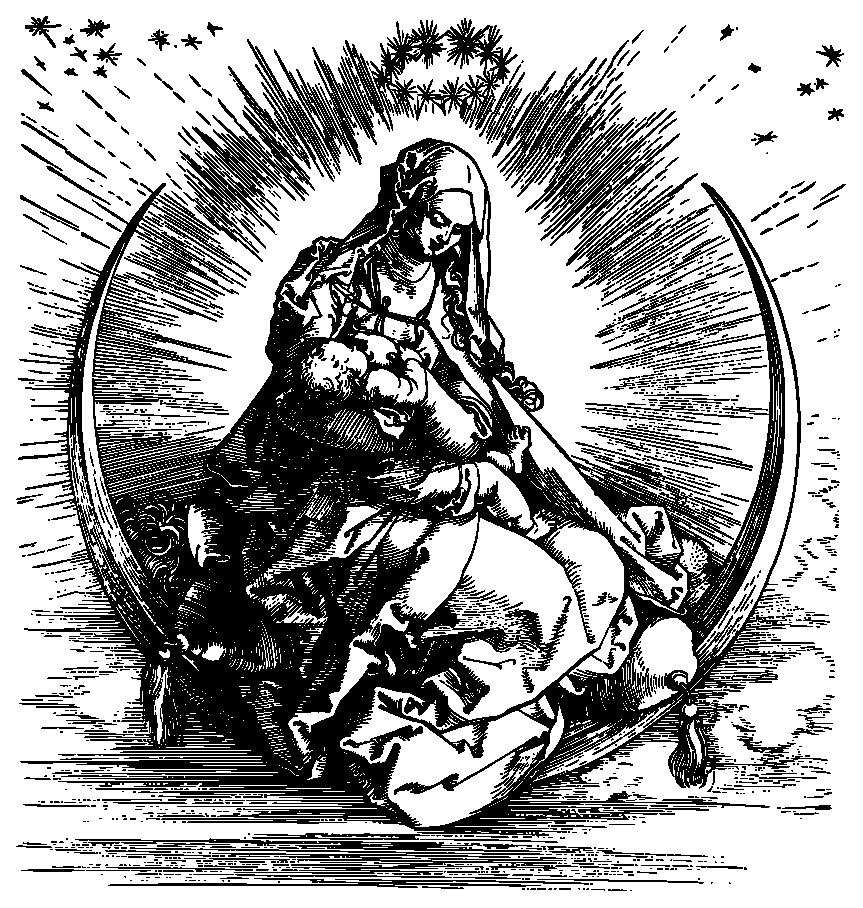
\includegraphics[scale=0.2]{tailpiece/MadonnaChildMoon.eps}
  \end{figure}


%MANUAL ADJUSTMENT:
\clearpage
\subsection{Absolution of the Dead}     
% \begin{rubric}
%     At the end of the Requiem Mass, the Celebrant retires to the Epistle Corner, where he takes off his chasuble and maniple, and puts on a black cope. The Subdeacon, between two Acolytes with lighted candles, carries the cross as in Processions, two other Acolytes preceding them, one with the thurible and incense-boat, the other with the aspersorium and aspergilium. The Celebrant follows, having first made a reverence to the Altar, with the Deacon on his left. The Subdeacon with the Cross takes his stand at the feet of the bier or catafalque opposite the altar, between the aforesaid Acolytes holding candles, while the Celebrant stands on the other side at the head of the place between the Altar and the bier, turning a little towards the Epistle corner, so that he looks towards the Subdeacon's Cross; on his left the Deacon, and near him the two other Acolytes carrying the thurible and aspersorium. Then, an Acolyte or Clerk holding the book, the Celebrant says at once the following Collect no change of number or sex being made, even if it is said for many persons or a woman: which Collect, however, is omitted if the body be not present.
% \end{rubric}\par
\begin{rubric}
	If this office follow a Requiem Mass, the Priest takes off his chasuble and maniple, and puts on a black cope. He then proceeds to stand at the foot of the bier, where he says the following prayer.
\end{rubric}


\lett{E}{nter} not into judgment with thy servant, O Lord, for in thy sight shall no man living be justified, except thou grant unto him remission of all his sins. Therefore, we beseech thee, let not the sentence of thy judgment fall upon him, whom the faithful prayer of Christian people commendeth unto thee: but by the succour of thy grace let him who while he lived was sealed with the sign of the Holy Trinity be found worthy to escape the avenging judgment: Who livest and reignest world without end. \textit{Amen.}

\begin{rubric}
    Then, the Cantor beginning, the Clerks standing around sing the following Responsory:
\end{rubric}\par\noindent
Deliver me, O Lord, * from death eternal in that fearful day: * When the heavens and the earth shall be shaken: * When thou shalt come to judge the world by fire. ℣. I am in fear and trembling till the sifting be upon us, and the wrath to come, * When the heavens and the earth shall be shaken. ℣. O that day that day of anger, of calamity and misery, a great day and exceeding bitter. * When thou shalt come to judge the world by fire. ℣. Rest eternal grant unto them, O Lord: and let light perpetual shine upon them.\par
℟. Deliver me, O Lord, * from death eternal in that fearful day: * When the heavens and the earth shall be shaken: * When thou shalt come to judge the world by fire.

\begin{rubric}
    Towards the end of the Responsory, the Celebrant puts incense into the thurible, blessing it as usual, the Deacon ministering the boat.
\end{rubric}
\begin{rubric}
	The Responsory ended, the Priest says,
\end{rubric}

℣. Lord, have mercy upon us.

℟. Christ, have mercy upon us.

℣. Lord, have mercy upon us.

%\begin{rubric}
%    Then the Priest says in a loud voice: \emph{Our Father}, the rest being said secretly by all. Meanwhile the Priest receives the aspergilium from the hand of the Deacon, and makes a reverence to the Altar; the Deacon accompanying him on his right, and holding the fore-edge of the Cope, he makes the circuit of the bier, sprinkling it with Holy Water, thrice on the right side and thrice on the left. When he passes in front of the Cross be bows low, while the Deacon genuflects: afterwards be receives the thurible from the Deacon, and censes the bier in the same manner as he has sprinkled it. Having returned to his first position, the Deacon holding the book, he says with joined hands:
%\end{rubric}
\begin{rubric}
	While the Lord's Prayer is said silently, the Priest goeth about the bier, sprinkling it with Holy Water, thrice on each side; and then in like manner he censes it, thrice on each side. He then says aloud,
\end{rubric}
℣. And lead us not into temptation.

℟. But deliver us from evil.\\

℣. From the gate of hell.

℟. Deliver \textit{his} soul, O Lord.

℣. May \textit{he} rest in peace.

℟. Amen.

℣. O Lord, hear my prayer.

℟. And let my cry come unto thee.

℣. The Lord be with you.

℟. And with thy spirit.

℣. Let us pray.
\par\noindent
	\centerline{\rule{0.5\textwidth}{0.4pt}}
\par\noindent
\begin{rubric}
	If the Body be present, the following Collect shall be said.
\end{rubric}
\lett{O}{God,} whose property is ever to have mercy and to forgive, we humbly entreat thee for the soul of thy \textit{servant} \textit{N.}, which thou hast this day commanded to depart from this world: deliver it not into the hands of the enemy, neither forget it at the last, but command that it be received by thy holy Angels, and brought unto the fatherland of paradise; that forasmuch as \textit{he} hoped and believed in thee, \textit{he} may not undergo the pains of hell, but may obtain everlasting felicity. Through Christ, our Lord. \textit{Amen.}
\par\noindent
	\centerline{\rule{0.5\textwidth}{0.4pt}}
\par\noindent
\begin{rubric}
	If the Body be not present, the following shall be said.
\end{rubric}
\lett{A}{bsolve,} O Lord, we beseech thee, the \textit{soul} of thy \textit{servant} \textit{N.} from every bond of sin: that in the glory of the resurrection, \textit{he} may be raised up amid thy Saints and elect unto newness of life. Through Christ, our Lord. \textit{Amen.}

\begin{rubric}
    Then, the Priest making a cross with his right hand over the bier, says,
\end{rubric}

℣. Rest eternal grant unto \textit{him,} O Lord.

℟. And let light perpetual shine upon \textit{him}.

℣. May \textit{he} rest in peace.

℟. Amen.\par

\begin{rubric}
    The Celebrant, again making a cross over the bier, says without inflexion:
\end{rubric}
℣. May \textit{his} soul and the souls of all the faithful departed through the mercy of God rest in peace.

℟. Amen.
\par\noindent
	\centerline{\rule{0.5\textwidth}{0.4pt}}
\par\noindent

%MANUAL ADJUSTMENT:
\clearpage
\subsection{Service at the Grave}

\begin{rubric}
	While the Body is being borne from the Church to the Grave, the following shall be sung,
\end{rubric}

 \lett{I}{nto} Paradise * may the Angels lead thee: at thy coming may the Martyrs receive thee, and bring thee into the holy city Jerusalem. May the Choirs of Angels receive thee, and with Lazarus, once poor, mayest thou have eternal rest.

\subsubsection{Blessing of the Grave}
\begin{rubric}
    If the ground be unconsecrated, when the Priest and People arrive, the following blessing is said.
\end{rubric}
\letuspray
%From the 1929 Scottish BCP:
\lett{O}{Lord} Jesu Christ, who wast laid in the new tomb of Joseph, and didst thereby sanctify the grave to be a bed of hope to thy people: Vouchsafe, we beseech thee, to bless, ha {\ding{64}} llow, and consecrate this grave, that it may be a resting-place, peaceful and secure, for the body of thy servant which we are about to commit to thy gracious keeping; who art the resurrection and the life, and who livest and reignest with the Father and the Holy Ghost, one God, world without end. \textit{Amen.}
\begin{rubric}
    The Priest then sprinkles the grave with Holy Water, and then censes the Body and the Grave.
\end{rubric}

\subsubsection{At the Grave}
\begin{rubric}
    When they come to the Grave, while the Body is made ready to be laid into the earth, shall be sung or said,
\end{rubric}\par

\lett{M}{an,} that is born of a woman, hath but a short time to live, and is full of misery. He cometh up, and is cut down, like a flower; he fleeth as it were a shadow, and never continueth in one stay.\par
\secondline{In the midst of life we are in death; of whom may we seek for succour, but of thee, O Lord, who for our sins art justly displeased?}
\thirdline{Yet, O Lord God most holy, O Lord most mighty, O holy and most merciful Saviour, deliver us not into the bitter pains of eternal death.}
    Thou knowest, Lord, the secrets of our hearts; shut not thy merciful ears to our prayer; but spare us, Lord most holy, O God most mighty, O holy and merciful Saviour, thou most worthy Judge eternal, suffer us not, at our last hour, for any pains of death, to fall from thee.
\begin{inhead}
    or,
\end{inhead}
\lett{A}{ll} that the Father giveth me shall come to me: and him that cometh to me I will in no wise cast out.\par
    \secondline{He that raised up Jesus from the dead: will also quicken your mortal bodies by the spirit which dwelleth in you.}
    \thirdline{Wherefore my heart is glad, and my glory rejoiceth: my flesh also shall rest in hope.}
    Thou shalt show me the path of life; in thy presence is the fulness of joy: and at thy right hand there is pleasure for evermore.

\begin{rubric}
    Then, while the earth shall be cast upon the Body by some standing by, the Priest shall say,
\end{rubric}

\lett{U}{nto} Almighty God we commend the soul of our \textit{brother} departed, and we commit \textit{his} body to the ground; earth to earth, ashes to ashes, dust to dust; in sure and certain hope of the Resurrection unto eternal life, through our Lord Jesus Christ, at whose coming in glorious majesty to judge the world, the earth and the sea shall give up their dead; and the corruptible bodies of those who sleep in him shall be changed, and made like unto his own glorious body; according to the mighty working whereby he is able to subdue all things unto himself.

\begin{rubric}
    Then shall be said or sung,
\end{rubric}\par\noindent
\antiphon{}{I heard a voice from heaven, saying unto me, Write, From henceforth blessed are the dead who die in the Lord: even so saith the Spirit; for they rest from their labours.}

\lett{B}{lessed} {\ding{64}} be the Lord God of Israel; * for he hath visited and redeemed his people;\par
    \secondline{And hath raised up a mighty salvation for us, * in the house of his servant David;}
    \thirdline{As he spake by the mouth of his holy Prophets, * which have been since the world began;}
    That we should be saved from our enemies, * and from the hand of all that hate us.\par
    To perform the mercy promised to our forefathers, * and to remember his holy covenant;\par
    To perform the oath which he sware to our forefather Abraham, * that he would give us;\par
    That we being delivered out of the hand of our enemies * might serve him without fear;\par
    In holiness and righteousness before him, * all the days of our life.\par
    And thou, child, shalt be called the prophet of the Highest: * for thou shalt go before the face of the Lord to prepare his ways;\par
    To give knowledge of salvation unto his people * for the remission of their sins,\par
    Through the tender mercy of our God; * whereby the day-spring from on high hath visited us;\par
    To give light to them that sit in darkness, and in the shadow of death, * and to guide our feet into the way of peace.

℣. Rest eternal * grant unto them, O Lord.\par
℟. And let light perpetual * shine upon them.

\antiphon{}{I heard a voice from heaven, saying unto me, Write, From henceforth blessed are the dead who die in the Lord: even so saith the Spirit; for they rest from their labours.}\\

℣. The Lord be with you.

℟. And with thy spirit.

℣. Let us pray.

℣. Lord, have mercy upon us.

℟. Christ, have mercy upon us.

℣. Lord, have mercy upon us.

\lett{O}{ur} Father, who art in heaven, Hallowed be thy Name. Thy kingdom come. Thy will be done on earth, As it is in heaven. Give us this day our daily bread. And forgive us our trespasses, As we forgive those who trespass against us. And lead us not into temptation; But deliver us from evil. Amen.

\begin{rubric}
    Meanwhile, the Priest sprinkles the body with Holy Water.
\end{rubric}
%Taking from the English Ritual and providing a rubric for it:
\begin{rubric}
	Then the Priest shall say that which followeth.
\end{rubric}
\lett{G}{rant,} we beseech thee, O Lord, this mercy to thy \textit{servant} departed; that, forasmuch as \textit{he} desired to do thy will, \textit{he} may not suffer the punishment of \textit{his} misdeed: that, as true faith joined \textit{him} to the company of the faithful here below, so in heaven thy mercy may number \textit{him} among the angelic choirs. Through Christ, our Lord. \textit{Amen.}
\begin{rubric}
    The Priest may say one or more of the following Prayers, at his discretion.
\end{rubric}\par

\lett{O}{God,} whose mercies cannot be numbered; Accept our prayers on behalf of the soul of thy \textit{servant} departed, and grant \textit{him} an entrance into the land of light and joy, in the fellowship of thy saints; through Jesus Christ our Lord. \textit{Amen.}\par

\lett{A}{lmighty} God, with whom do live the spirits of those who depart hence in the Lord, and with whom the souls of the faithful, after they are delivered from the burden of the flesh, are in joy and felicity; We give thee hearty thanks for the good examples of all those thy servants, who, having finished their course in faith, do now rest from their labours. And we beseech thee, that we, with all those who are departed in the true faith of thy holy Name, may have our perfect consummation and bliss, both in body and soul, in thy eternal and everlasting glory; through Jesus Christ our Lord. \textit{Amen.}\par

\lett{O}{merciful} God, the Father of our Lord Jesus Christ, who is the Resurrection and the Life; in whom whosoever believeth, shall live, though he die; and whosoever liveth, and believeth in him, shall not die eternally; who also hath taught us, by his holy Apostle Saint Paul, not to be sorry, as men without hope, for those who sleep in him; We humbly beseech thee, O Father, to raise us from the death of sin unto the life of righteousness; that, when we shall depart this life, we may rest in him; and that, at the general Resurrection in the last day, we may be found acceptable in thy sight; and receive that blessing, which thy well-beloved Son shall then pronounce to all who love and fear thee, saying, Come, ye blessed children of my Father, receive the kingdom prepared for you from the beginning of the world. Grant this, we beseech thee, O merciful Father, through Jesus Christ, our Mediator and Redeemer. \textit{Amen.}\par

\lett{T}{he} God of peace, who brought again from the dead our Lord Jesus Christ, the great Shepherd of the sheep, through the blood of the everlasting covenant; Make you perfect in every good work to do his will, working in you that which is well pleasing in his sight; through Jesus Christ, to whom be glory for ever and ever. \textit{Amen.}

\lett{O}{almighty} God, the God of the spirits of all flesh, who by a voice from heaven didst proclaim, Blessed are the dead who die in the Lord; Multiply, we beseech thee, to those who rest in Jesus, the manifold blessings of thy love, that the good work which thou didst begin in them may be perfected unto the day of Jesus Christ. And of thy mercy, O heavenly Father, vouchsafe that we, who now serve thee here on earth, may at last, together with them, be found meet to be partakers of the inheritance of the saints in light; for the sake of the same thy Son Jesus Christ our Lord. \textit{Amen.}\par

\lett{M}{ost} merciful Father, who hast been pleased to take unto thyself the soul of this thy servant; Grant to us who are still in our pilgrimage, and who walk as yet by faith, that having served thee with constancy on earth, we may be joined hereafter with thy blessed saints in glory everlasting; through Jesus Christ our Lord. \textit{Amen.}\par

\lett{O}{Lord} Jesus Christ, who by thy death didst take away the sting of death; Grant unto us thy servants so to follow in faith where thou hast led the way, that we may at length fall asleep peacefully in thee, and awake up after thy likeness; through thy mercy, who livest with the Father and the Holy Ghost, one God, world without end. \textit{Amen.}\par

\lett{A}{lmighty} and everliving God, we yield unto thee most high praise and hearty thanks, for the wonderful grace and virtue declared in all thy saints, who have been the choice vessels of thy grace, and the lights of the world in their several generations; most humbly beseeching thee to give us grace so to follow the example of their stedfastness in thy faith, and obedience to thy holy commandments, that at the day of the general Resurrection, we, with all those who are of the mystical body of thy Son, may be set on his right hand, and hear that his most joyful voice: Come, ye blessed of my Father, inherit the kingdom prepared for you from the foundation of the world. Grant this, O Father, for the sake of the same, thy Son Jesus Christ, our only Mediator and Advocate. \textit{Amen.}\par
\begin{rubric}
	The Priest then continues,
\end{rubric}
℣. Rest eternal grant unto \textit{him}, O Lord.\par
℟. And let light perpetual shine upon \textit{him}.\par
℣. May \textit{he} rest in peace.\par
℟. Amen.

\lett{M}{ay} \textit{his} soul, {\ding{64}} and the souls of all the faithful departed, through the mercy of God, rest in peace. \textit{Amen.}

\lettspace

\begin{rubric}
    The Priest then sprinkles the grave with Holy Water.
\end{rubric}
\par\noindent
	\centerline{\rule{0.5\textwidth}{0.4pt}}
\par\noindent
\subsection{At the Burial of the Dead at Sea}
\begin{rubric}
    The same office may be used; but instead of the Sentence of Committal, the Minister shall say,
\end{rubric}\par

\lett{U}{nto} Almighty God we commend the soul of our brother departed, and we commit his body to the deep; in sure and certain hope of the Resurrection unto eternal life, through our Lord Jesus Christ; at whose coming in glorious majesty to judge the world, the sea shall give up her dead; and the corruptible bodies of those who sleep in him shall be changed, and made like unto his glorious body; according to the mighty working whereby he is able to subdue all things unto himself.